% ----------------------------------------------------------
% Metodologia
% ----------------------------------------------------------
\chapter{Metodologia} \label{cha:metodologia}

Este capítulo apresenta a metodologia adotada no desenvolvimento deste trabalho, descrevendo as etapas e os procedimentos utilizados na pesquisa. Para alcançar os objetivos propostos, a execução do projeto foi estruturada nas seguintes etapas:

Inicialmente, será realizada uma revisão bibliográfica sobre a indústria de jogos digitais, desenvolvimento colaborativo, design de interface e usabilidade, com o objetivo de fundamentar a pesquisa e levantar os requisitos da plataforma. Em seguida, serão definidos os fluxos de navegação e elaborados protótipos de baixa e alta fidelidade, permitindo validar a organização das telas e a experiência do usuário.

Por fim, o protótipo de interface será implementado utilizando tecnologias de desenvolvimento, aplicando princípios de usabilidade, acessibilidade e \textit{design} centrado no usuário, serão também realizados testes para verificar o fluxo de navegação e o funcionamento das principais funcionalidades da interface.

\begin{figure}[htbp]
    \centering
    \caption{Fluxograma metodológico do desenvolvimento do projeto.}
    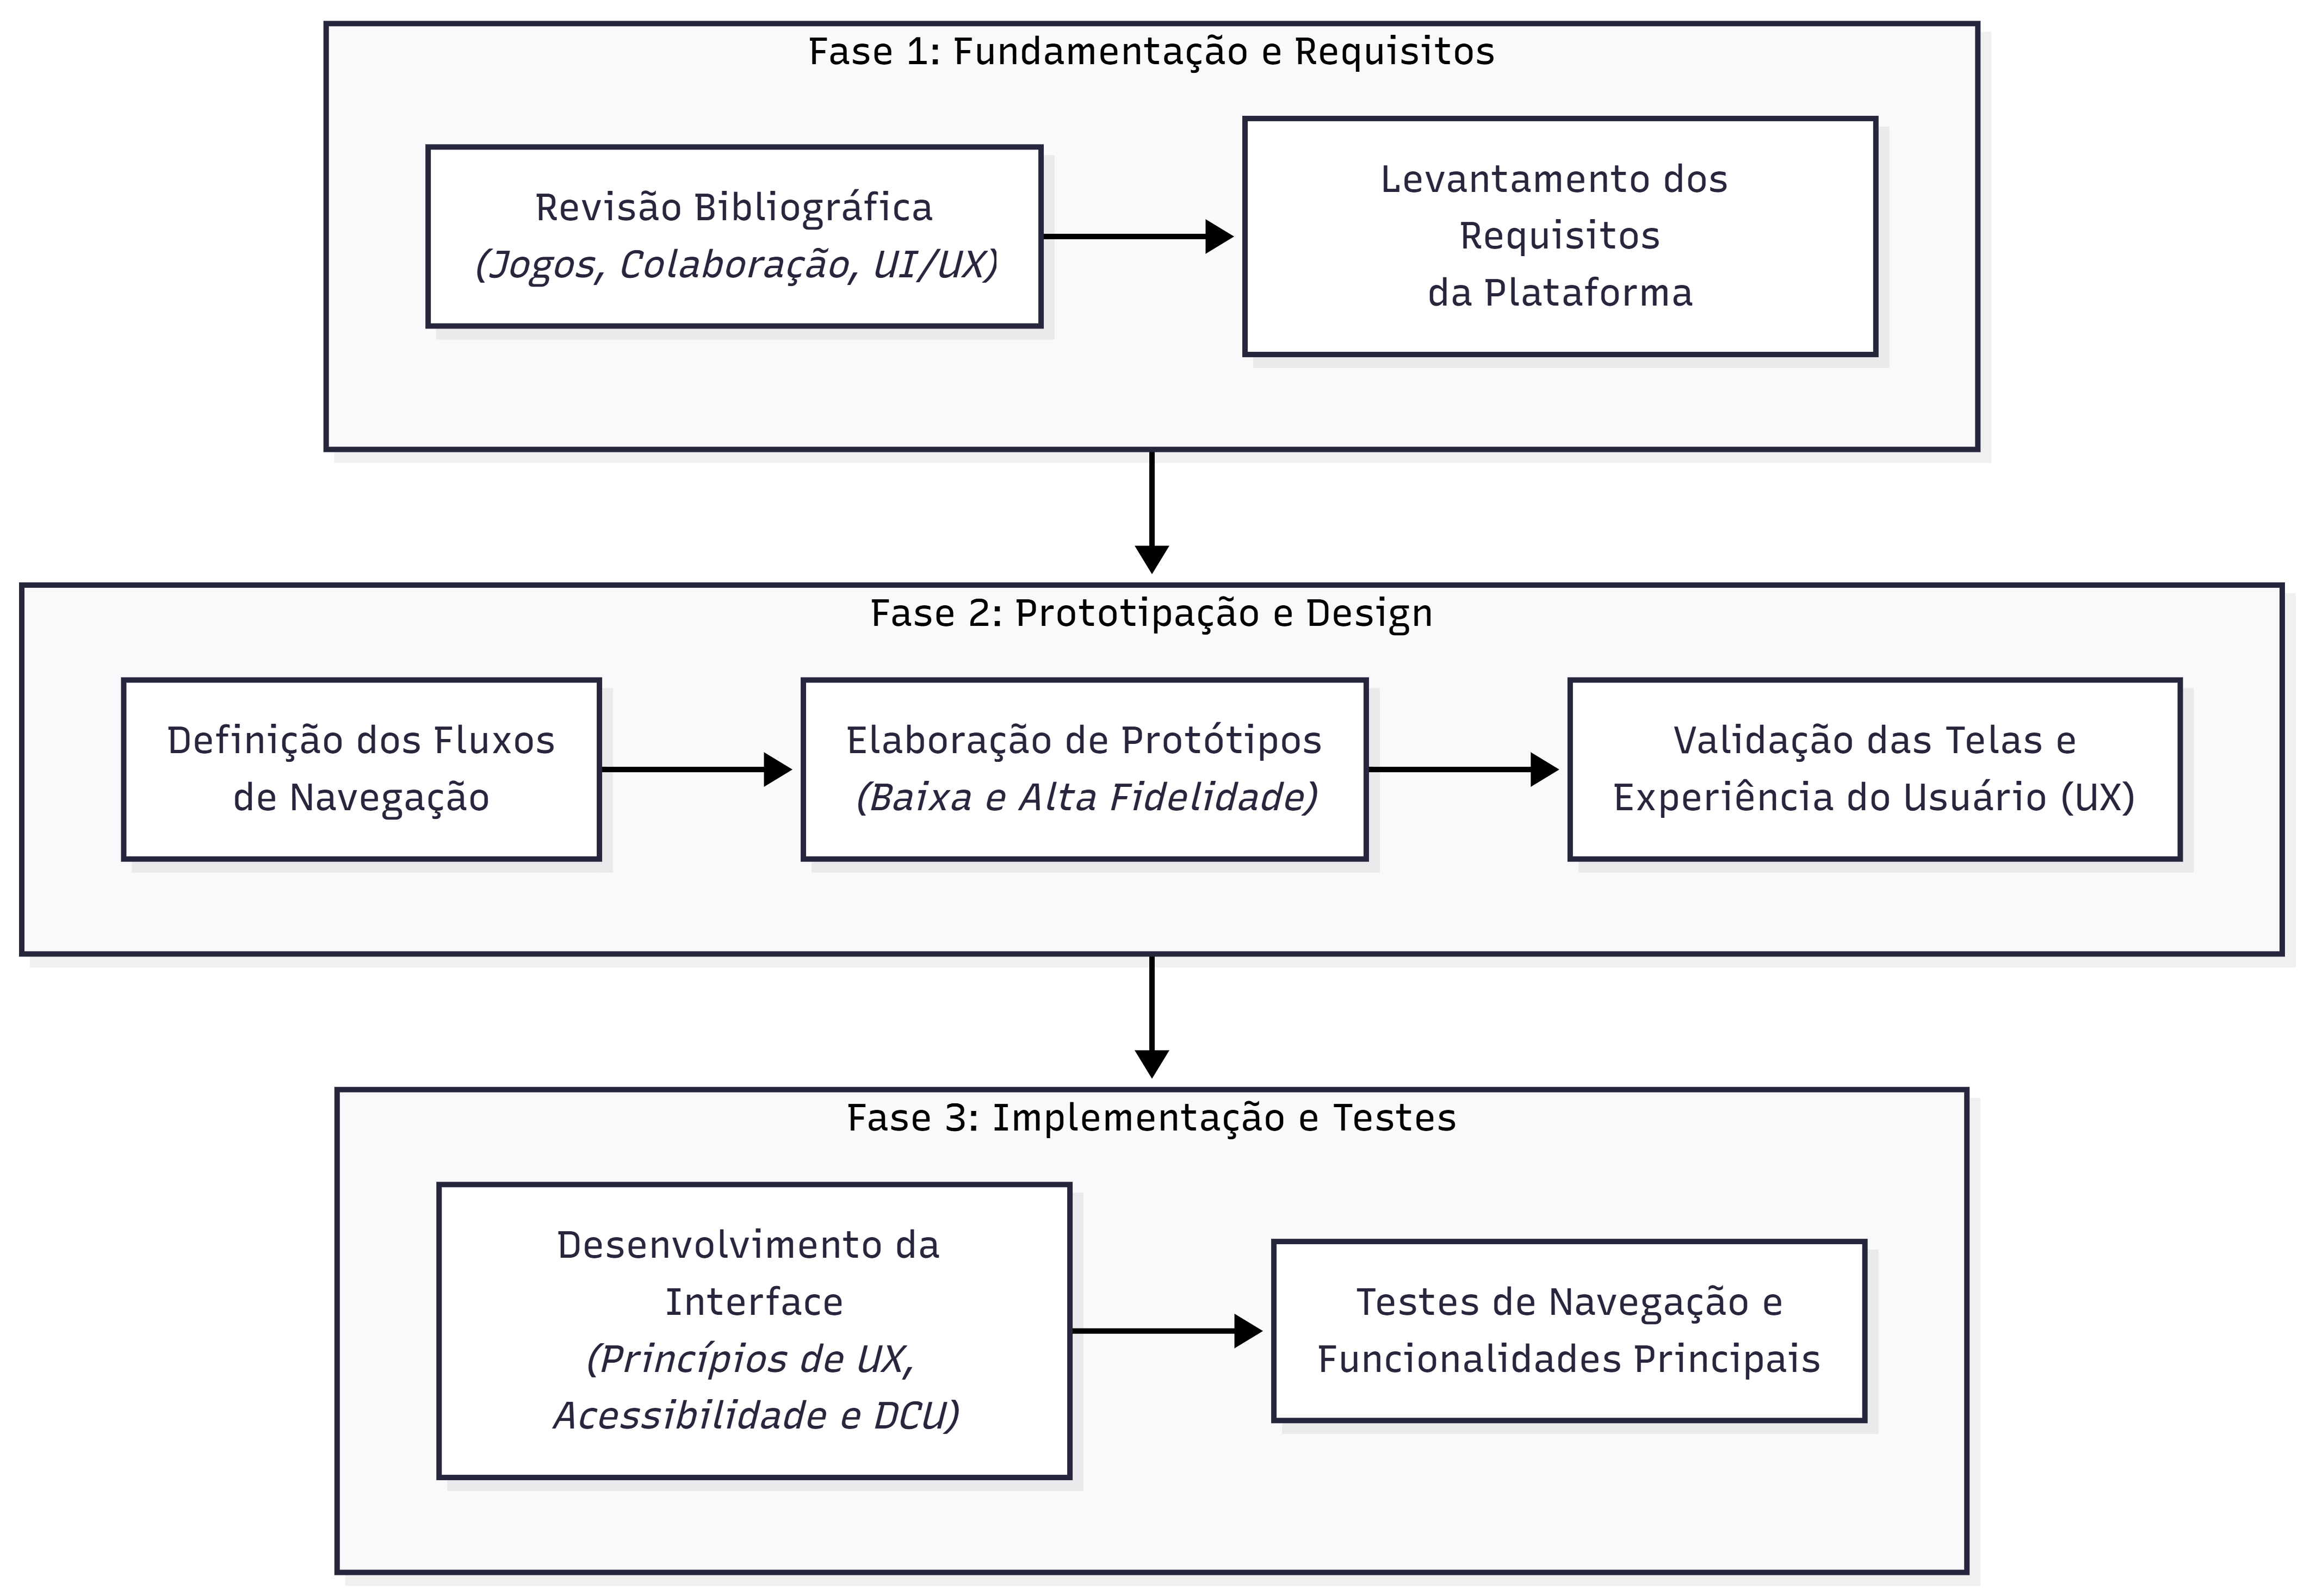
\includegraphics[width=0.85\textwidth]{imagens/fluxograma_metodologia.png}
    \label{fig:fluxo_metodologico}
    \small
    \\[0.1cm]
    \textbf Fonte: Elaborado pela autora (2026).
\end{figure}